\documentclass[a4paper,12pt]{article} 
\usepackage[T1]{fontenc} 
\usepackage{enumerate}
\usepackage{graphicx}
\usepackage{listings}
\usepackage{subfigure}
\usepackage[a4paper,top=2.5cm,bottom=2.5cm,left=2.5cm,right=2.5cm]{geometry}


\title{\bf Features extraction and image clustering}
\date {19 January 2015}
\author{Lorenzo Cioni, Francesco Santoni\\\textit{{\small lore.cioni@gmail.com, fsanto92@hotmail.it}}}

\begin{document}
\maketitle

\begin{abstract}
In this report we will discuss a method of extracting features from manostritti characters in order of clustering similar words that represent the American States from census of 1970.
\end{abstract}

\tableofcontents

\section{Introduction}
Segmentation and clustering of large amounts of data is one of the main research fields of modern artificial intelligence.

The basis of our work is the collection of u.s. Census data in the year 1940 and fits into the process of digitalizing of handwritten documents that characterizes our time. In this case we have scans of census register and the main problem is to divide enrollees for each American State.

Document segmentation and extraction of the word corresponding to the State was developed previously by two of our colleagues in the course of \emph{Technology of Databases} and is the base from which our work started.So the problem on which we have worked is the extraction of features from handwritten characters to cluster similar words in order to facilitate the recognition by a human agent.

\begin{figure}[!ht]
\centering
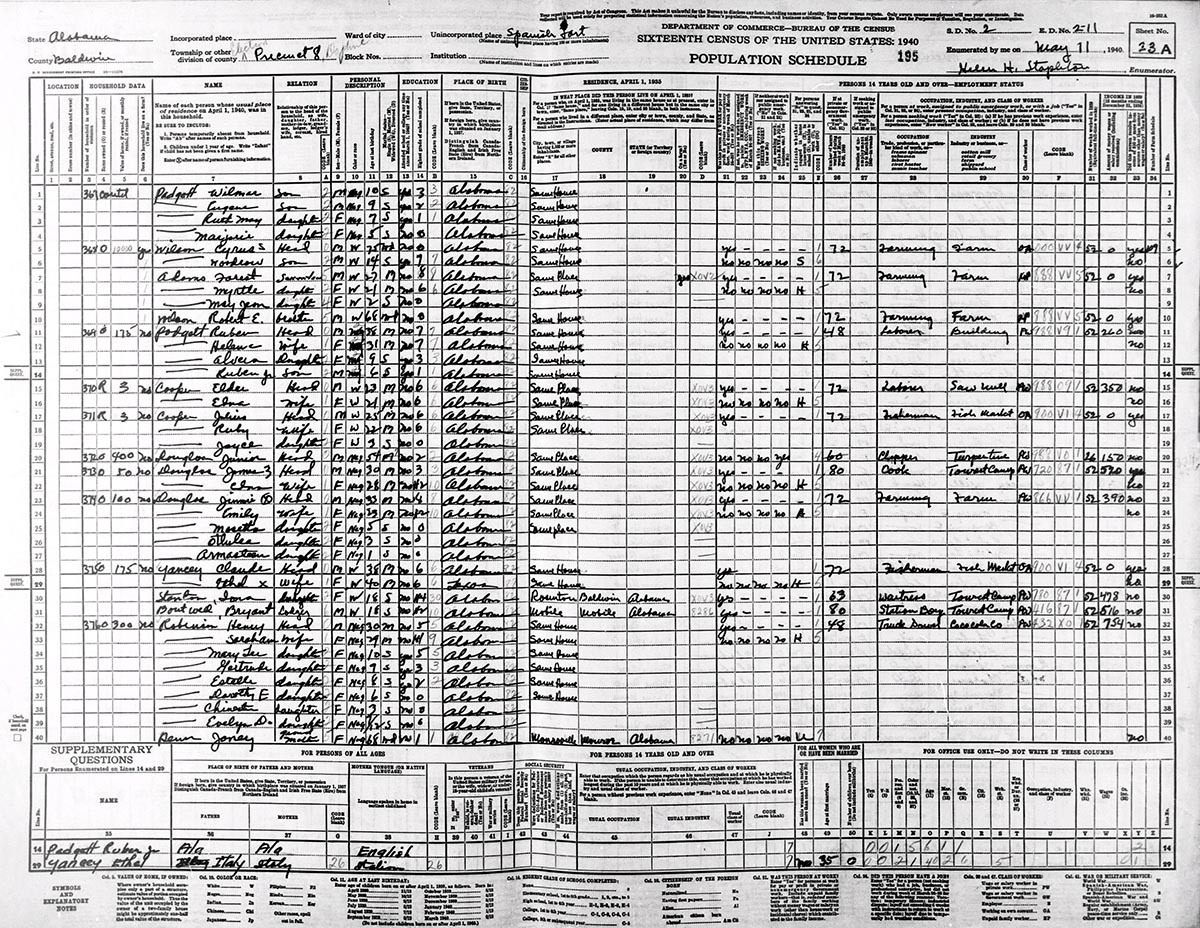
\includegraphics[width=0.6\textwidth]{images/img1.jpg}
\caption{An example of a table containing census data}
\end{figure}

\section{The project}

The page that contains the data in digital form, contains a wealth of information about each person surveyed including name, gender, membership status and some secondary features such as work or the breed. 

All these data are housed in a moulded grid composed of numbered rows and columns for each field to conduct a census. In addition to the data of persons are reported on each archive also additional data related to censor or data relating to samples of the population.

The objective of the project was concerned with finding a particular grid area, the State of each person, from which extract handwritten text associated with the correct name of the State.

Following the data extraction, the project plans to group visually similar elements to form a collection of homogenous States. So each set and then will contain grid theoretically corresponding cutouts of the same State.

\subsection{Process steps}

We can summarize the project in three basic steps:
\begin{enumerate}
\item Search for the text area containing the words of interest
\item Row segmentation
\item Postprocessing of each cut image
\end{enumerate}

The last step, the clustering of images, is our point of interest: it has been rewritten and improved using new features extraction method and a new method for evaluating similarity and will be discussed in detail later.

\subsubsection{Word searching}

In this first phase the aim is to identify the region of the grid within which we find the State words. 

First of all we remove the black border of the document resulting from scanning. Then, using the technique of vertical histogram, we can locate the grid columns and, knowing the correct column's offset relative to the beginning of the document, just the one concerned is extracted is extracted.

\subsubsection{Row segmentation}

After the extraction of the column concerned from the document, we proceed with row segmentation.

Similar to the previous step, but using the histogram horizontal this time, we are able to determine with some accuracy the rows in the grid. In this case, however, was necessary to center the word in the extracted image: this is done by correcting the height of each row by the analysis of black spikes on the histogram.

At the end of this phase, each word is contained in a single image.

\subsubsection{Postprocessing}

In this postprocessing phase the individual images extracted are reworked in order to remove any  vertical or horizontal residual lines from the previous cut.

Delete row/column strokes can be about as bring back the black pixels related to the residual value of pure white (255 as grayscale).

This allows us to extract the most significant features in the next steps of processing.

\begin{figure}[!ht]
\centering
\vspace{0.3cm}
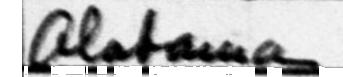
\includegraphics[width=0.5\textwidth]{images/img2.jpg}
\caption{An image extracted from document.}
\label{fig:extracted_image}
\end{figure}

As you can see in Figure \ref{fig:extracted_image}, the word is centered and the extra line have been removed (there is a line set to white). For each picture we proceed with feature extraction for handwritten characters and clustering. 

\subsection{Troubles}

The identification of words and their segmentation and has some strong issues.

A first problem is represented by the document skew. In this case, this may be due to a not perfectly horizontal scan of the original document. The presence of skew reduces the performance in searching for rows and columns of the grid, thus making impossible segmentation. In some cases, for example, is interpreted incorrectly the first column and this causes the extraction of the wrong column in the first stage of the process.

The main problems of the second phase are mainly related to the identification of extraneous lines. Because of the large number of dashed lines present isn't always possible to \emph{clean} the images and this can cause errors in clustering.

\begin{figure}[!ht]
 \centering
 \subfigure[An image with a dashed line]
   {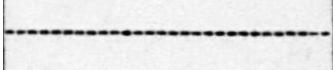
\includegraphics[width=0.3\textwidth]{images/img3.jpg}}
 \hspace{5mm}
 \subfigure[The line intersects the word]
   {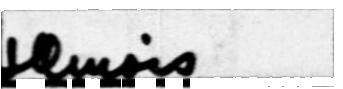
\includegraphics[width=0.3\textwidth]{images/img4.jpg}}
 \caption{Segmentation and postprocessing issues}
 \end{figure}

In other cases the word intersects directly gridlines. Because of this we may experience a loss of information about words by removing the line using the method described above.


\section{Clustering}

The clustering phase provides for the categorization of the various segments in homogeneous groups, so that, at the end of the process, each of them have the same words.

At this stage the main goal is to be able to extract some good features from images that will be used for comparison. The aim is to construct a similarity matrix between different segments so that they can be used as input to the clustering algorithm.

Unable to establish a priori the final number of desired clusters is used \emph{Affinity Propagation}.

\subsection{Features}

% % pezzo su come sono fatte stringhe


In this work we want to find \emph{primitive} features, resembling the possible types of strokes used to write a word, to characterize the sample from which they are extracted in order to perform clustering on their set.

The features are identified by the study of a sub-portion, or window, of the images extracted by the paper on which this work is based.

The features are located through a study of an area, the window, to which they are implicitly associated: as such there is no clear order of which of the features found in the area comes first.
Due to the absence of such \emph{native} order the string that defines a window is maintained consistent with the other strings trough the convention of generating the string with the features' identifiers always taking the same order, if present.

The chosen way to resolve the issue however presents the problem of making sliding windows inapplicable: this means that a sample must necessarily be cut in separate windows, which are allowed to overlap, with the corresponding effect that due to the random cut some features like \textit{loops} may not be recognised in an instance and recognised in another. 

\paragraph{Windows}

Currently we have chosen to cut the samples in windows of 32 pixels each with the exception of the last part of the sample that, deemed irrelevant to the end of characterization due to containing almost always white space, is simply ignored.

These windows are spaced only 16 pixels from the preceding and succeeding one, with the intent of creating overlap and lengthening the string that characterizes the samples.

While the simplest way to create the windows is simply creating a new PIX with the required coordinates it requires unnecessary passages and time in the creation of new objects. We have thus preferred to increase the complexity of the functions that search for the features, to whom we pass as a variable the original sample PIX with information about the \textit{offset} at which to start the search and the \textit{width} of the window.

% %parte su diversa width diverse feature

\subsubsection{Whitespace}  

The first feature that is search in the windows is the white space. This way if a window is identified as blank will not be necessary to proceed with the investigation of other features, saving time.

A window is identified as blank if the average pixel values is below a preset white threshold.

\subsubsection{Loop}

The feature that represents a loop is recognized only with maximum window size.
To locate a loop is initially found a black pixel. The idea behind is to imagine that we had found a point on the border and meet two transitions going in the same direction, first from black to white then from white to black. Between the two transitions there must be a minimum step above a preset threshold where the pixels are white.

If the above condition occurs then we verify that it is real in the same way along the horizontal axis. We then sit in the center of the loop (the median value of the segment described above) and check that, moving both right or left you get a transition from white to black after a suitable number of white pixels.

The implemented method has numerous problems related mainly to the identification of the center of the loop in the segment. With a value of threshold too high also might have to discard some loops too small. The method also does not take into account the thickness of the stroke.
However, with appropriate threshold values you can get good results and to identify obvious loops of various segments.

\subsubsection{Dot}

\subsubsection{Diagonal line}
The feature representing a diagonal line, both upward and downward facing, is extracted through a simple exhaustive scansion of the window for lines of connected black pixels that have an incline in a range of values and are sufficiently long.

At the moment the function doesn't account for the width of the lines found, thus diagonal features can be recognised in a shapeless blob of black pixel that is sufficiently big. 
   
There's a distinction for diagonal features that appear in the lower and upper bottom of the window.
At most in a window the function identifies a couple of upward and a couple of downward facing lines (lower and upper parts), once one has been found it stops searching for the same type.

Of these couples the function search searchs then if they possibly intersects, in such a case a \emph{crossing} feature is extracted too, with distinction if the crossing happens in the lower or upper part. 

\subsubsection{Horizontal and Vertical line}
Both horizontal and vertical lines' features are extracted through
a simple scan of the window.
The horizontal lines requires a double-window for their implicit characteristic.
The function identifies a line if it finds a connected row or column of black pixels that has sufficient length, in particular it distinguishes the lines found in normal or long through an ulterior threshold.
Once a fitting line has been found the function keeps searching for more, continuing the scansion of the window after having moved a certain distance from the last line found in order not to confuse a particularly thick stroke as different separate lines.
There still persists the problem that the stroke width is not fully considered so a big blob of black pixels is seen as a series of horizontal and vertical lines, at the same time such an occurrence is rare so the presence of many horizontal and vertical lines ends up distinguishing the word in itself.     

\subsubsection{Cross}  
  
\subsection{LCS} 

In order to compare the generated strings each others we use the \emph{Longest Common Subsequence} (LCS) algorithm for evaluating distances.

 
 
\subsection{Affinity Propagation}

\section{Results}

\section{Conclusion} 


\end{document}